\documentclass{article}

\usepackage[margin=1in]{geometry}
\usepackage{xcolor}
\usepackage{listings}
\usepackage{enumitem}
\usepackage{booktabs}
\usepackage[hidelinks]{hyperref}
\usepackage{tikz}
\usetikzlibrary{arrows.meta, positioning, shapes.geometric, fit, backgrounds, calc}

\definecolor{codebg}{RGB}{245,245,245}
\definecolor{codekw}{RGB}{0,90,180}
\definecolor{codecom}{RGB}{110,110,110}
\definecolor{codestr}{RGB}{160,30,30}

\lstdefinelanguage{JS}{
  keywords={const, let, var, function, return, if, else, for, while, import, export, from, default, new, this, of, in, class, extends, true, false, null, undefined},
  keywordstyle=\color{codekw}\bfseries,
  sensitive=true,
  comment=[l]{//},
  morecomment=[s]{/*}{*/},
  string=[b]',
  morestring=[b]",
  morestring=[b]`,
}

\lstdefinestyle{js}{
  language=JS,
  backgroundcolor=\color{codebg},
  basicstyle=\ttfamily\footnotesize,
  keywordstyle=\color{codekw}\bfseries,
  commentstyle=\color{codecom}\itshape,
  stringstyle=\color{codestr},
  showstringspaces=false,
  breaklines=true,
  frame=single,
  numbers=left,
  numberstyle=\tiny\color{gray},
  tabsize=2,
}

\title{Matter.js: Implementing Hot Restart}
\author{Adan Rodriguez}
\date{\today}

\begin{document}
\maketitle

\tableofcontents

\section{Background: where this left off}

The earlier note in this document (see the previous draft) observed the
following behavior when saving a file during development:

\begin{quote}
\itshape
On save, the compiler rebuilds and \texttt{webpack-hot-middleware} pushes
the update over the webpack HMR SSE stream. The client checks whether any
module in the update chain called \texttt{.accept()} --- none did --- so it
logs \texttt{"[HMR] ... do not know how to hot reload themselves ...
(Full reload needed)"} and stops. Because \texttt{reload} is \texttt{false},
it does not auto-refresh either. The page sits there unchanged until a
human manually hits refresh.
\end{quote}

Two remediation paths were identified: (1) wire up real
\texttt{module.hot.accept()} / \texttt{module.hot.dispose()} handling around
the render loop, being careful not to stack duplicate loops on repeated
updates, or (2) a simpler \texttt{reload=true} query-string override that
forces a full page reload on every save. This document implements path (1),
specifically the \emph{hot restart} variant of it: on every accepted
update, the previous simulation is fully torn down and a fresh one is
built, rather than trying to preserve in-flight physics state across edits.

\section{The change}

\subsection{Before}

\begin{lstlisting}[style=js]
const render = (context, engine) => {
  clearCanvas(context, CANVAS_WIDTH, CANVAS_HEIGHT);
  drawBodies(context, engine.world.bodies);
  requestAnimationFrame(() => render(context, engine));
};

const main = (() => {
  const { Engine, Runner, Bodies, Composite } = Matter;

  const engine = Engine.create();
  Composite.add(engine.world, createWorldBodies(Bodies));

  const canvas = createCanvas(CANVAS_WIDTH, CANVAS_HEIGHT);
  const context = getContext2d(canvas);
  mountCanvas(canvas);

  const runner = Runner.create();
  Runner.run(runner, engine);

  render(context, engine);
})();
\end{lstlisting}

\texttt{main} is an anonymous, self-invoking function expression (IIFE). It
runs exactly once, at module-evaluation time, and everything it creates
(\texttt{engine}, \texttt{canvas}, \texttt{runner}) is scoped inside its
closure --- nothing outside can reach them. \texttt{render} recurses through
\texttt{requestAnimationFrame} without ever storing the frame id it
receives, so the loop cannot be cancelled from outside itself.

\subsection{After}

\begin{lstlisting}[style=js]
let engine, runner, canvas, rafId;

const render = (context, engine) => {
  clearCanvas(context, CANVAS_WIDTH, CANVAS_HEIGHT);
  drawBodies(context, engine.world.bodies);
  rafId = requestAnimationFrame(() => render(context, engine));
};

const start = () => {
  const { Engine, Runner, Bodies, Composite } = Matter;

  engine = Engine.create();
  Composite.add(engine.world, createWorldBodies(Bodies));

  canvas = createCanvas(CANVAS_WIDTH, CANVAS_HEIGHT);
  const context = getContext2d(canvas);
  mountCanvas(canvas);

  runner = Runner.create();
  Runner.run(runner, engine);

  render(context, engine);
};

const stop = () => {
  Matter.Runner.stop(runner);
  cancelAnimationFrame(rafId);
  canvas.remove();
};

start();

if (module.hot) {
  module.hot.dispose(stop);
  module.hot.accept();
}
\end{lstlisting}

\subsection{Logical explanation of each change}

\begin{description}[leftmargin=1.6cm, style=nextline]
  \item[Module-level state] \texttt{engine}, \texttt{runner}, \texttt{canvas}
    and \texttt{rafId} move from \texttt{const}s trapped inside the IIFE's
    closure to \texttt{let} bindings at module scope. This is the
    prerequisite for everything else: a \texttt{dispose} callback that runs
    later, outside \texttt{start}, must be able to see and act on the exact
    instances \texttt{start} created.
  \item[\texttt{main} $\rightarrow$ \texttt{start}] The IIFE becomes a named,
    callable function. An IIFE runs once by construction; a restart strategy
    needs to invoke setup again, so setup has to be a function with a name,
    not a value produced by immediately invoking one.
  \item[\texttt{rafId} capture] \texttt{render} now assigns its own
    \texttt{requestAnimationFrame} return value to the module-level
    \texttt{rafId} on every frame. Previously this id was discarded, so
    there was no way to stop the animation loop from outside; now
    \texttt{stop} can call \texttt{cancelAnimationFrame(rafId)} against the
    most recent pending frame.
  \item[\texttt{stop}] A new function performing full, unconditional
    teardown: stop the physics \texttt{Runner} (halts the fixed-timestep
    physics ticks), cancel the pending animation frame (halts the draw
    loop), and remove the mounted \texttt{<canvas>} from the DOM. Note that
    \texttt{Runner} is referenced as \texttt{Matter.Runner} here rather than
    the destructured local from \texttt{start} --- the destructured binding
    only exists inside \texttt{start}'s scope, so \texttt{stop} must go
    through the \texttt{Matter} namespace import directly.
  \item[\texttt{module.hot.dispose(stop)}] Registers \texttt{stop} as the
    cleanup callback for \emph{this instance} of the module. Webpack's HMR
    runtime guarantees this callback runs immediately before the replacement
    module executes, and never any earlier --- so the old simulation is torn
    down exactly once, right before the new one starts.
  \item[\texttt{module.hot.accept()}] Called with no arguments, this
    self-accepts updates to \emph{this} module. It tells the HMR runtime
    "when this module (or anything importing it up to here) changes, don't
    bubble the update further up the module graph or fall back to a full
    page reload --- just re-execute this module in place." Because
    \texttt{start()} is called unconditionally at the bottom of the file,
    re-executing the module is what performs the actual restart: a brand
    new \texttt{Engine}, brand new bodies at their original coordinates from
    \texttt{createWorldBodies}, a brand new canvas.
\end{description}

This is a \emph{restart}, not a state-preserving \emph{reload}: no attempt
is made to save body positions, velocities, or any other simulation state
across an edit. Every accepted save produces a scene identical to a hard
refresh, but without the browser navigating away, reconnecting the
dev-server socket, or re-fetching the full HTML document.

\section{Execution model}

\subsection{Cold start (first page load)}

\begin{enumerate}
  \item The browser requests \texttt{/}; Express responds with
    \texttt{dist/index.html} (generated by \texttt{HtmlWebpackPlugin}, which
    already references \texttt{main.bundle.js}).
  \item The browser requests \texttt{main.bundle.js}; the webpack runtime
    boots, evaluates \texttt{src/index.js} for the first time.
  \item At the bottom of the module, \texttt{module.hot} exists (because
    \texttt{HotModuleReplacementPlugin} is active and the entry includes
    \texttt{webpack-hot-middleware/client}), so \texttt{module.hot.dispose}
    and \texttt{module.hot.accept} are called --- but \texttt{stop} has not
    run yet, since nothing has been replaced.
  \item \texttt{start()} has already run synchronously just above that
    block, so the canvas is mounted and the render/physics loops are live.
\end{enumerate}

\subsection{Hot restart (save while the dev server is running)}

\begin{enumerate}
  \item A source file changes on disk.
  \item Webpack's compiler (running in watch mode inside
    \texttt{webpack-dev-middleware}) recompiles only the affected modules
    and computes an update chain.
  \item \texttt{webpack-hot-middleware} pushes a \texttt{hash} event, then
    the browser client requests the small \texttt{*.hot-update.json}
    manifest and the \texttt{*.hot-update.js} chunk containing the new
    module code.
  \item The webpack runtime in the browser walks the module graph looking
    for an accept handler. It finds \texttt{module.hot.accept()} was called
    by \texttt{src/index.js} itself, so the update chain terminates there
    --- no reload is needed, and the update does not have to bubble to
    \texttt{index.js}'s importers (there are none in this app).
  \item Before swapping in the new module factory, the runtime invokes every
    registered \texttt{dispose} callback for modules being replaced ---
    here, \texttt{stop()}: the \texttt{Runner} halts, the pending animation
    frame is cancelled, the old \texttt{<canvas>} is removed from the DOM.
  \item The new module code executes in place of the old one, which means
    \texttt{start()} runs again: fresh \texttt{Engine}, fresh bodies, fresh
    canvas mounted, fresh runner and render loop --- and the new
    \texttt{module.hot.dispose}/\texttt{accept} pair is registered for the
    \emph{next} save.
\end{enumerate}

\section{How webpack talks to the browser}

Two independent express middlewares are layered in \texttt{app.js} to make
this possible: \texttt{webpack-dev-middleware} handles serving compiled
assets from memory, and \texttt{webpack-hot-middleware} handles notifying
the browser when new assets are ready.

\begin{figure}[h]
\centering
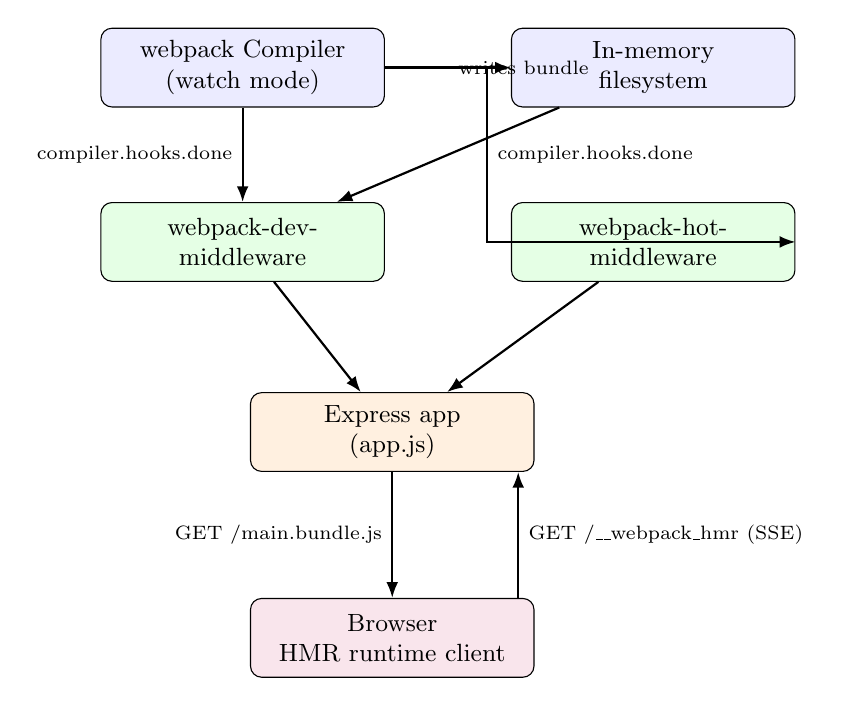
\begin{tikzpicture}[
  box/.style={draw, rounded corners, minimum width=3.6cm, minimum height=1cm, align=center, font=\small},
  arrow/.style={-{Latex[length=2mm]}, thick},
  node distance=1.2cm and 1.6cm
]
  \node[box, fill=blue!8] (compiler) {webpack Compiler\\(watch mode)};
  \node[box, fill=blue!8, right=of compiler] (memfs) {In-memory\\filesystem};
  \node[box, fill=green!10, below=of compiler] (devmw) {webpack-dev-\\middleware};
  \node[box, fill=green!10, right=of devmw] (hotmw) {webpack-hot-\\middleware};
  \node[box, fill=orange!12, below=1.4cm of devmw, xshift=1.9cm] (express) {Express app\\(app.js)};
  \node[box, fill=purple!10, below=1.6cm of express] (browser) {Browser\\HMR runtime client};

  \draw[arrow] (compiler) -- node[right, font=\scriptsize]{writes bundle} (memfs);
  \draw[arrow] (memfs) -- (devmw);
  \draw[arrow] (compiler) -- node[left, font=\scriptsize]{compiler.hooks.done} (devmw);
  \draw[arrow] (compiler.east) -- ++(1.3,0) |- node[near start, right, font=\scriptsize]{compiler.hooks.done} (hotmw.east);
  \draw[arrow] (devmw) -- (express);
  \draw[arrow] (hotmw) -- (express);
  \draw[arrow] (express.south) -- node[left, font=\scriptsize]{GET /main.bundle.js} (browser.north);
  \draw[arrow] ($(browser.north)+(1.6,0)$) -- node[right, font=\scriptsize]{GET /\_\_webpack\_hmr (SSE)} ($(express.south)+(1.6,0)$);
\end{tikzpicture}
\caption{Two middlewares wrap the same compiler instance: one serves files, the other streams update notifications.}
\end{figure}

\begin{itemize}
  \item \textbf{webpack-dev-middleware} owns the compiler's watch cycle. It
    keeps the latest build in an in-memory filesystem (no assets are written
    to \texttt{dist/} on disk in the request path) and answers ordinary
    asset requests (\texttt{main.bundle.js}, \texttt{index.html}) straight
    out of that memory, always the freshest build --- this is why the
    server does not need restarting when source changes.
  \item \textbf{webpack-hot-middleware} listens to the same compiler's
    \texttt{done} hook. On every successful recompilation it opens/keeps a
    Server-Sent-Events stream at \texttt{/\_\_webpack\_hmr} and pushes a
    small JSON event (essentially: \emph{"new build hash X is ready"}).
  \item The browser-side half of \texttt{webpack-hot-middleware}
    (\texttt{webpack-hot-middleware/client}, injected because it is
    prepended to the \texttt{main} entry in \texttt{webpack.config.js}) is
    what actually holds that SSE connection open, requests the
    \texttt{hot-update.json}/\texttt{hot-update.js} pair when notified, and
    hands them to webpack's HMR runtime (\texttt{module.hot.\{accept,
    dispose\}}, \texttt{\_\_webpack\_require\_\_.hmrM}, etc.) to apply.
\end{itemize}

\section{How Express talks to webpack}

\texttt{app.js} does not run webpack as a separate CLI process; it imports
the webpack config directly and drives the compiler in-process:

\begin{lstlisting}[style=js]
const compiler = webpack(webPackConfig);
const app = express();

app.use(webpackDevMiddleware(compiler));
app.use(webpackHotMiddleware(compiler));
app.use(express.static(path.join(__dirname, 'dist'), { index: false }));

app.get('/', (req, res) => {
  res.sendFile(path.join(__dirname, 'dist', 'index.html'));
});
\end{lstlisting}

\begin{figure}[h]
\centering
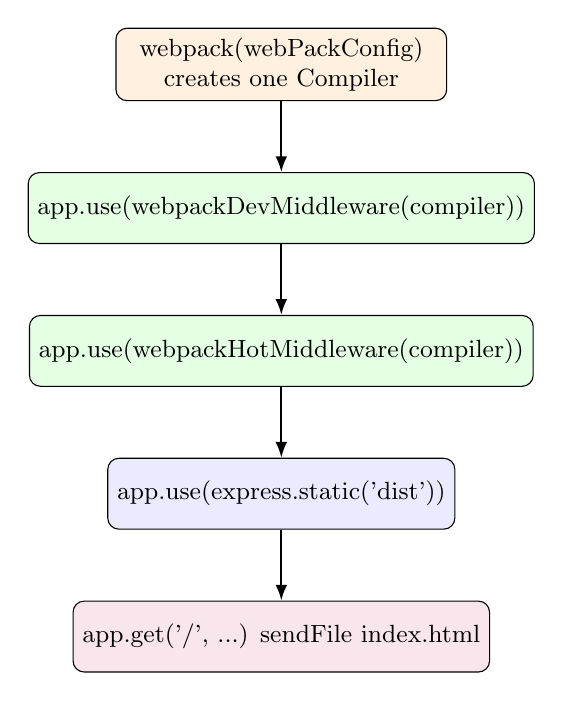
\begin{tikzpicture}[
  box/.style={draw, rounded corners, minimum width=4.2cm, minimum height=0.9cm, align=center, font=\small},
  arrow/.style={-{Latex[length=2mm]}, thick},
  node distance=0.9cm
]
  \node[box, fill=orange!12] (b1) {webpack(webPackConfig)\\creates one Compiler};
  \node[box, fill=green!10, below=of b1] (b2) {app.use(webpackDevMiddleware(compiler))};
  \node[box, fill=green!10, below=of b2] (b3) {app.use(webpackHotMiddleware(compiler))};
  \node[box, fill=blue!8, below=of b3] (b4) {app.use(express.static('dist'))};
  \node[box, fill=purple!10, below=of b4] (b5) {app.get('/', ...) sendFile index.html};

  \draw[arrow] (b1) -- (b2);
  \draw[arrow] (b2) -- (b3);
  \draw[arrow] (b3) -- (b4);
  \draw[arrow] (b4) -- (b5);
\end{tikzpicture}
\caption{Express middleware order in \texttt{app.js}. Both HMR middlewares share the \emph{same} compiler instance, which is what lets them coordinate on one build.}
\end{figure}

\texttt{webpack(webPackConfig)} only builds a \texttt{Compiler} object; it
does not compile anything by itself. Handing that one compiler to both
\texttt{webpack-dev-middleware} and \texttt{webpack-hot-middleware} is what
lets them stay in sync: the dev-middleware starts the compiler's watch loop
and exposes its output, and the hot-middleware taps into the lifecycle hooks
of that exact same compiler to know when a new build is ready to announce.
If two separate \texttt{webpack(...)} calls were used instead, the two
middlewares would be watching unrelated builds and would drift out of sync.
\texttt{express.static} and the explicit \texttt{/} route are the fallback
path for anything the dev-middleware does not intercept, and only matter
for the very first request (\texttt{index.html}) since dev-middleware
already answers for \texttt{main.bundle.js} and the hot-update files.

\section{Sequence diagram: a hot-restart round trip}

\begin{figure}[p]
\centering
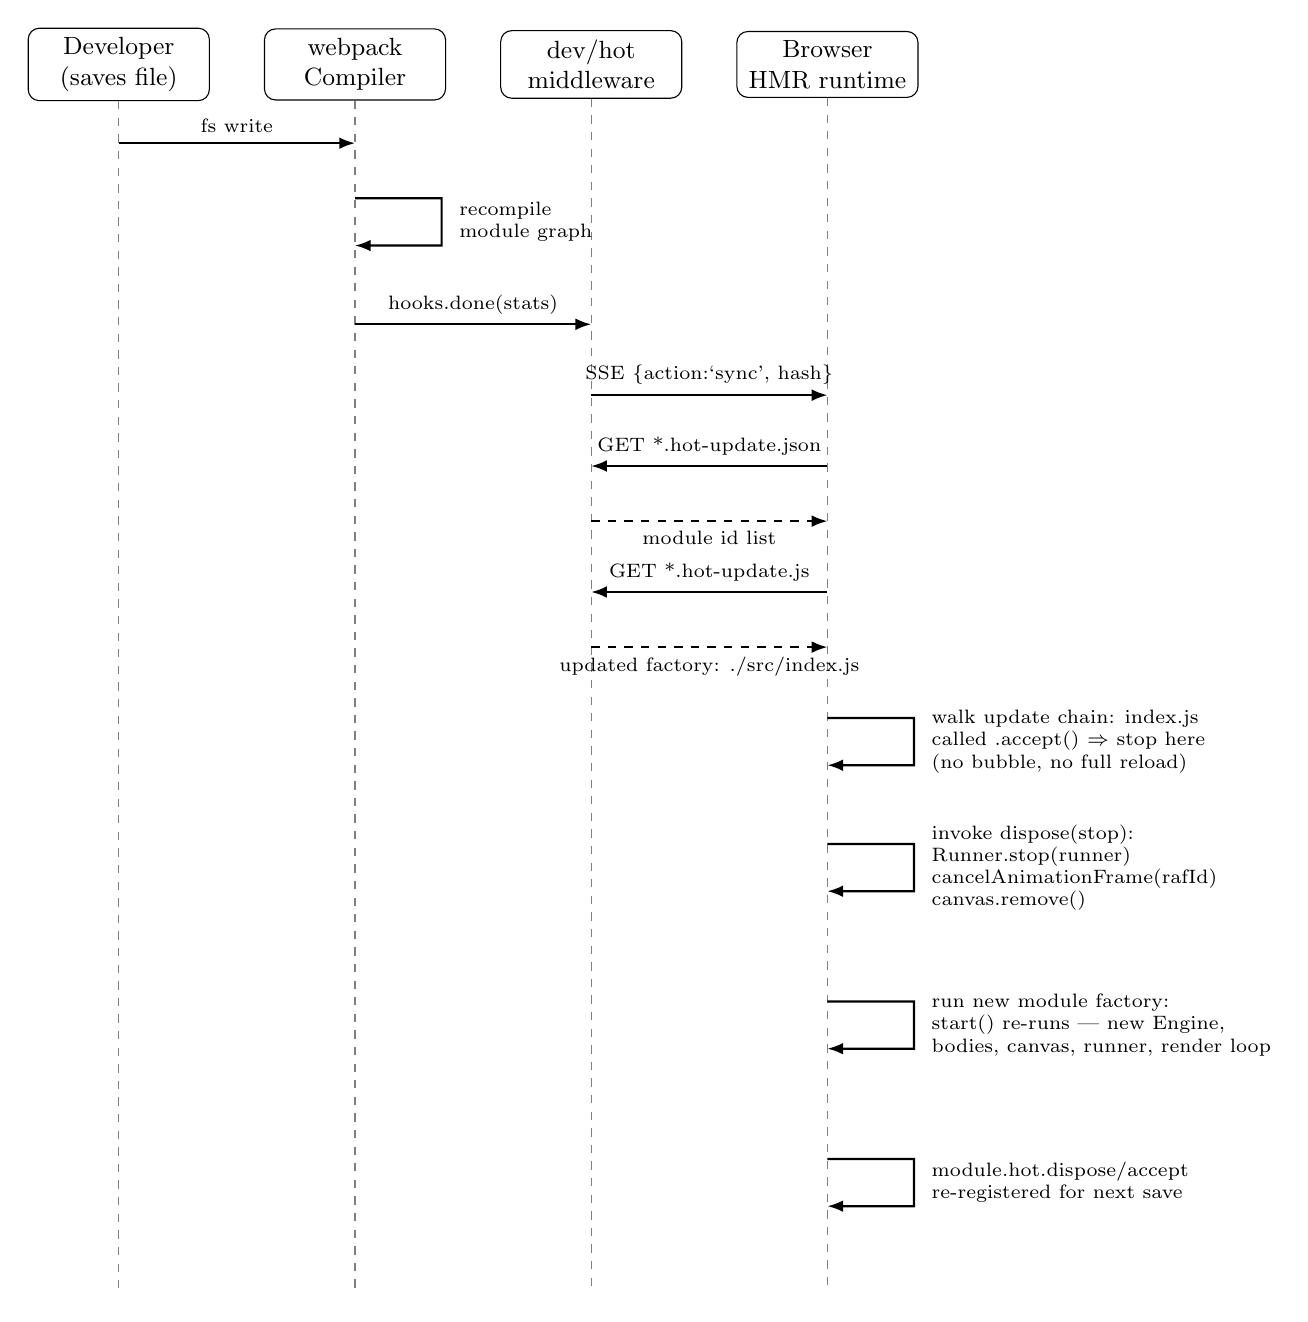
\begin{tikzpicture}[
  actor/.style={draw, rounded corners, minimum width=2.3cm, minimum height=0.7cm, align=center, font=\small},
  lifeline/.style={dashed, gray},
  msg/.style={-{Latex[length=2mm]}, thick, font=\scriptsize},
  msgret/.style={-{Latex[length=2mm]}, thick, dashed, font=\scriptsize},
  note/.style={font=\scriptsize, align=left}
]
  \def\devx{0}
  \def\compx{3.0}
  \def\mwx{6.0}
  \def\brx{9.0}
  \def\loopw{1.1}
  \def\ytop{0}
  \def\ybot{-15.6}

  \node[actor] (dev) at (\devx,\ytop) {Developer\\(saves file)};
  \node[actor] (comp) at (\compx,\ytop) {webpack\\Compiler};
  \node[actor] (mw) at (\mwx,\ytop) {dev/hot\\middleware};
  \node[actor] (br) at (\brx,\ytop) {Browser\\HMR runtime};

  \draw[lifeline] (dev.south) -- (\devx,\ybot);
  \draw[lifeline] (comp.south) -- (\compx,\ybot);
  \draw[lifeline] (mw.south) -- (\mwx,\ybot);
  \draw[lifeline] (br.south) -- (\brx,\ybot);

  \draw[msg] (\devx,-1.0) -- node[above]{fs write} (\compx,-1.0);

  \draw[msg] (\compx,-1.7) -- ++(\loopw,0) -- ++(0,-0.6) -- (\compx,-2.3);
  \node[note, anchor=west] at (\compx+\loopw+0.1,-2.0) {recompile\\module graph};

  \draw[msg] (\compx,-3.3) -- node[above]{hooks.done(stats)} (\mwx,-3.3);
  \draw[msg] (\mwx,-4.2) -- node[above]{SSE \{action:`sync', hash\}} (\brx,-4.2);

  \draw[msg] (\brx,-5.1) -- node[above]{GET *.hot-update.json} (\mwx,-5.1);
  \draw[msgret] (\mwx,-5.8) -- node[below]{module id list} (\brx,-5.8);

  \draw[msg] (\brx,-6.7) -- node[above]{GET *.hot-update.js} (\mwx,-6.7);
  \draw[msgret] (\mwx,-7.4) -- node[below]{updated factory: ./src/index.js} (\brx,-7.4);

  \draw[msg] (\brx,-8.3) -- ++(\loopw,0) -- ++(0,-0.6) -- (\brx,-8.9);
  \node[note, anchor=west] at (\brx+\loopw+0.1,-8.6) {walk update chain: index.js\\called .accept() $\Rightarrow$ stop here\\(no bubble, no full reload)};

  \draw[msg] (\brx,-9.9) -- ++(\loopw,0) -- ++(0,-0.6) -- (\brx,-10.5);
  \node[note, anchor=west] at (\brx+\loopw+0.1,-10.2) {invoke dispose(stop):\\Runner.stop(runner)\\cancelAnimationFrame(rafId)\\canvas.remove()};

  \draw[msg] (\brx,-11.9) -- ++(\loopw,0) -- ++(0,-0.6) -- (\brx,-12.5);
  \node[note, anchor=west] at (\brx+\loopw+0.1,-12.2) {run new module factory:\\start() re-runs --- new Engine,\\bodies, canvas, runner, render loop};

  \draw[msg] (\brx,-13.9) -- ++(\loopw,0) -- ++(0,-0.6) -- (\brx,-14.5);
  \node[note, anchor=west] at (\brx+\loopw+0.1,-14.2) {module.hot.dispose/accept\\re-registered for next save};
\end{tikzpicture}
\caption{End-to-end timeline from file save to the DOM showing a freshly restarted simulation.}
\end{figure}

\section{Why this counts as a \emph{restart} and not a \emph{reload}}

Two different things are commonly called "hot reload," and this codebase
now implements the simpler of the two:

\begin{center}
\begin{tabular}{@{}p{3.6cm}p{5.6cm}p{5.6cm}@{}}
\toprule
 & \textbf{State-preserving reload} & \textbf{Hot restart (this change)} \\
\midrule
Simulation state across an edit & Kept (e.g. bodies keep their current position/velocity) & Discarded; scene resets to \texttt{createWorldBodies}' initial layout \\
\texttt{dispose} responsibility & Selectively serialize state into \texttt{module.hot.data} & Unconditionally stop everything: runner, rAF, DOM node \\
Complexity & Higher --- must reconcile old/new state shape when code changes & Lower --- next \texttt{start()} call is identical to a cold boot \\
Full page reload / socket reconnect & No & No \\
\bottomrule
\end{tabular}
\end{center}

Extending this into a true state-preserving reload later would only
require \texttt{stop} to stash whatever should survive (e.g. body positions)
onto \texttt{module.hot.data}, and \texttt{start} to read it back out if
present --- the \texttt{accept}/\texttt{dispose} wiring itself would not
change.

\end{document}
